\documentclass[12pt, a4paper]{article}

\usepackage{amsmath}

\usepackage{ntheorem}
% \theoremstyle{nonumberplain}
\theorembodyfont{\upshape}
\newtheorem{theorem}{Theorem}
% \newtheorem{proof}{Proof}[section]
\newenvironment{proof}{{\newline\noindent\bf Proof}\quad}{\hfill $\square$\par}

\usepackage{amsfonts}
\def\bbE{\mathbb{E}}
\def\bbX{\mathbb{X}}

\usepackage{graphicx}
\usepackage{pdfpages}
\usepackage[titletoc, title]{appendix}

\usepackage{hyperref}
\hypersetup{
    colorlinks=true,
    linkcolor=blue,
    filecolor=magenta,      
    urlcolor=cyan,
}


\def\vx{\boldsymbol{x}}
\def\vw{\boldsymbol{w}}
\def\vtheta{\boldsymbol{\theta}}

\def\rmx{\mathrm{x}}
\def\rmX{\mathrm{X}}

\def\vrmx{\boldsymbol{\mathrm{x}}}

\DeclareMathOperator*{\relu}{ReLU}
\DeclareMathOperator*{\argmax}{arg\,max}
\DeclareMathOperator*{\argmin}{arg\,min}

\newcommand{\expect}[3]{\mathbb{E}_{#1 \sim #2} \left[ #3 \right]}
\newcommand{\egx}[1]{\boldsymbol{x}^{(#1)}}
\newcommand{\dkl}[2]{D_{\mathrm{KL}}(#1 \Vert #2)}


\title{Information Theory}
\author{CHEN Si}
\date{}


\begin{document} 


\maketitle
\tableofcontents


\section{Introduction}

\begin{itemize}
    \item A branch of applied mathematics
    \item Fundamental to many areas of electrical engineering and computer science
\end{itemize}


\section{Goals}

\begin{itemize}
    \item In Electrical Engineering
        \begin{itemize}
            \item Quantify how much information is present in a signal 
            \item Tells how to design optimal codes and calculate the expected length of messages sampled from specific probability distributions using various encoding schemes
        \end{itemize}
    \item In Machine Learning
        \begin{itemize}
            \item Characterize probability distributions
            \item Quantify similarity between probability distributions
        \end{itemize}
\end{itemize}


\section{Self-Information}
\paragraph{Motivation}
\begin{itemize}
    \item To quantify the information of events
\end{itemize}

\paragraph{Intuition}
\begin{itemize}
    \item Likely events should have low information content
    \item Less likely events should have higher information content
    \item Independent events should have additive information
\end{itemize}

\paragraph{Definition (Discrete Random Variable)} 
The \textbf{self-information} of an event $\mathrm{x}=x$ is defined as
\[
    I(x) = - \log P(x)
\]
Units:
\begin{enumerate}
    \item \textbf{nats}: if $\log$ is the natural logarithm with base $e$
        \begin{itemize}
            \item One nat is the amount of information gained by observing an event of probability $\frac{1}{e}$
            \item In machine learning, we usually use nats
        \end{itemize}
    \item \textbf{bits} or \textbf{shannons}: if $\log$ is base-$2$
        \begin{itemize}
            \item Information measured in bits is just a rescaling of information measured in nats
        \end{itemize}
\end{enumerate}
\paragraph{Definition (Continuous Random Variable)} 
We use the same definition of information by analogy, but some of the properties from the discrete case are lost
\begin{itemize}
    \item e.g. An event with unit density still has zero information, despite not being an event that is guaranteed to occur
\end{itemize}


\section{Shannon Entropy}
\paragraph{Motivation}
\begin{itemize}
    \item To quantify the amount of uncertainty in an entire probability distribution
\end{itemize}

\paragraph{Definition}
\[
    H(P) = H(\rmx) = \bbE_{\rmx \sim P} [I(x)] = -\mathbb{E}_{\rmx \sim P}[\log P(x)]
\]
\begin{itemize}
    \item Gives a lower bound on the number of bits needed on average to encode symbols drawn from a distribution $P$
    \item Distributions taht are nearly deterministic (where the outcome is nearly certain) have low entropy; distributions that are closer to uniform have high entropy
    \item When $\rmx$ is continuous, the Shannon entropy is known as the \textbf{differential entropy}
\end{itemize}


\section{Kullback-Leibler (KL) divergence}
\paragraph{Motivation}
\begin{itemize}
    \item To measure how different two distributions (over the same random variable) are
\end{itemize}

\paragraph{Definition}
\[
    D_{KL}(P \Vert Q) = \bbE_{\rmx \sim P} \left[ \log \frac{P(x)}{Q(x)} \right] = \bbE_{\rmx \sim P} [\log P(x) - \log Q(x)]
\]
\begin{itemize}
    \item In the case of descrete variables, it is the extra amount of information needed to send a message containing symbols drawn from probability distribution $P$, when we use a code that was designed to minimize the length of messages drawn from probability distribution $Q$
\end{itemize}
\paragraph{Properties}
\begin{itemize}
    \item Non-negative (\hyperref[theo:dkl]{proof})
    \item The KL divergence is $0$ if and only if $P$ and $Q$ are the same distribution in the case of discrete variables, or equal "almost everywhere" in the case of continuous variables
    \item Similar to some sort of distance between these distributions, but it is not symmetric $D_{KL}(P \Vert Q) \neq D_{KL}(Q \Vert P)$
    \item The choice of whether to use $D_{KL}(P \Vert Q)$ or $D_{KL}(Q \Vert P)$ depends on requirements (see Appendix \ref{app:asy_kl} for details)
\end{itemize}


\section{Cross-Entropy}
\paragraph{Definition}
\[
    H(P, Q) = - \expect{\rmx}{P}{\log Q(x)}
\]
\paragraph{Properties}
\begin{itemize}
    \item $ H(P,Q) = H(P) + D_{KL}(P \Vert Q) $
    \item $\min\limits_Q H(P, Q) \Longleftrightarrow \min\limits_Q D_{KL}(P \Vert Q)$
    \item $0 \log 0 = \lim\limits_{x \to 0} x \log x = 0$ (by convention in information theory)
\end{itemize}


\newpage
\begin{appendices}
% \renewcommand{\appendixname}{Appendix~\Alph{section}}

\section{Asymmetry of KL divergence}
\label{app:asy_kl} 
\begin{enumerate}
    \item To minimize $\dkl{p}{q}$
        \begin{enumerate}
            \item $q(x)$ needs to be large when $p(x)$ is large
            \item $\dkl{p}{q}$ is not sensitive to q when $p(x)$ is small
        \end{enumerate}
    \item To minimize $\dkl{q}{p}$
        \begin{enumerate}
            \item $q(x)$ needs to be small when $p(x)$ is small
            \item $\dkl{q}{p}$ is not sensitive to q when $p(x)$ is large
        \end{enumerate}
\end{enumerate}
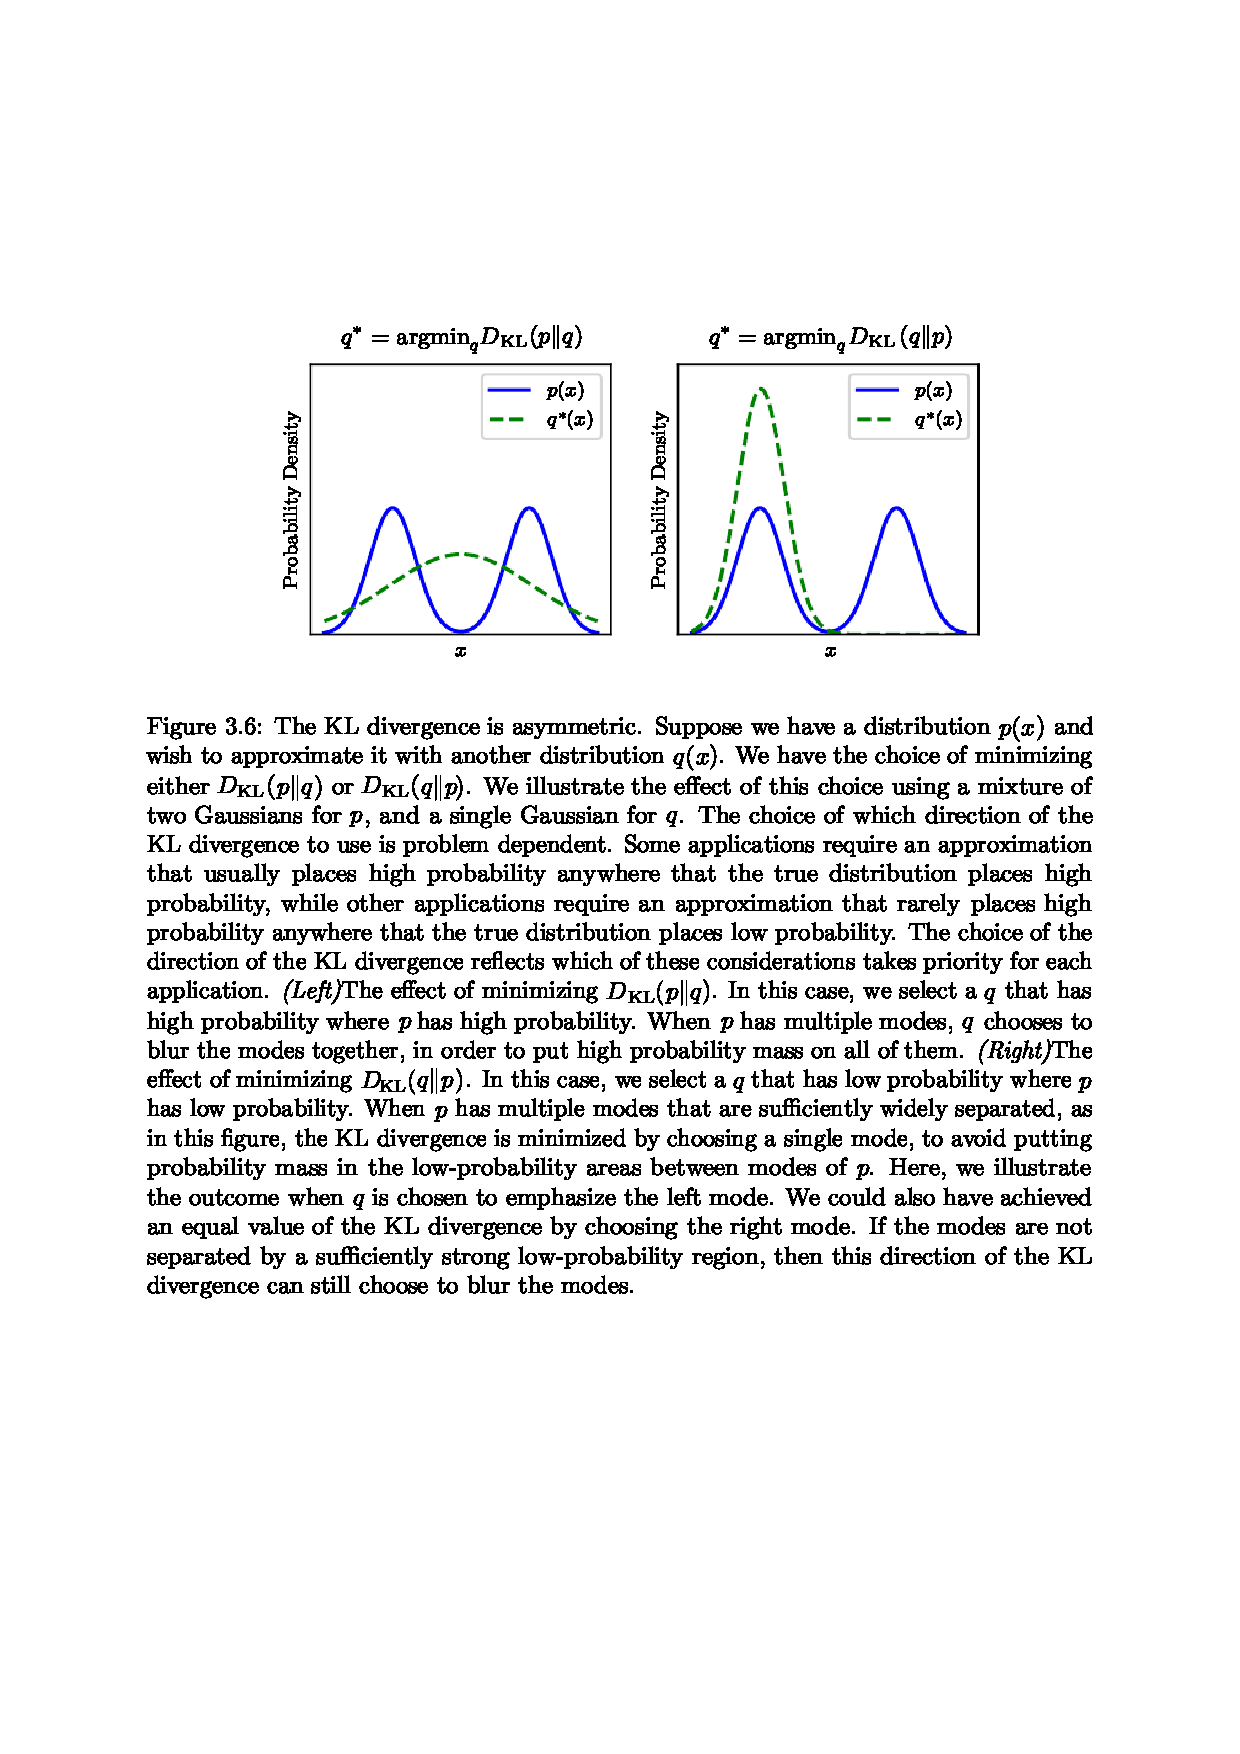
\includegraphics[width=\textwidth]{../imgs/Asymmetry_of_KL_divergence.pdf}


\section{Theorems \& Proofs}

\begin{theorem}[Jensen's Inequality]

    \label{theo:jensen}
    If $\rmX$ is a random variable and $f$ a convex function, then
    \[
        f(\mathbb{E}[\rmX]) \leq \mathbb{E}[f(\rmX)]
    \]
    Moreover, if $f$ is strictly convex, the equality in implies that $X = \mathbb{E}[X]$ with probability $1$ (i.e., $X$ is a constant).
    \newline
    \begin{proof}
        We prove this for discrete distributions by induction on the number of mass points.
        \begin{itemize}
            \item For a two-mass-point distribution, the inequality becomes
                \[
                    p_1 f(x_1) + p_2 f(x_2) \geq f(p_1x_1 + p_2x_2)
                \]
                which follows directly from the definition of convex functions.
            \item Suppose that the theorem is true for distributions with $k − 1$ mass points.
                Then writing $p'_i = p_i / (1 - p_k)$ for $i = 1, 2, \dots, k-1$, we have
                \[
                    \begin{split}
                        \sum_{i=1}^k p_i f(x_i) 
                        &= p_k f(x_k) + (1-p_k) \sum_{i=1}^{k-1} p'_i f(x_i)
                        \\&\geq p_k f(x_k) + (1-p_k) f \left( \sum_{i=1}^{k-1}p'_i x_i \right)
                        \\&\geq f \left( p_kx_k + (1-p_k)\sum_{i=1}^{k-1}p'_ix_i \right)
                        \\&= f \left( \sum_{i=1}^k p_ix_i \right)
                    \end{split}
                \]
        \end{itemize}
    \end{proof}

    (\href{https://en.wikipedia.org/wiki/Jensen%27s_inequality}{see more} for continous case)

\end{theorem}

\begin{theorem}[Information Inequality]
\label{theo:dkl}

    Let $p(x)$, $q(x)$, $x\in\mathcal{X}$, be two probability mass functions. Then
    \[
        \dkl{p}{q} \geq 0  
    \]
    with equality if and only if $p(x)=q(x)$ for all $x$.
    \newline\newline
    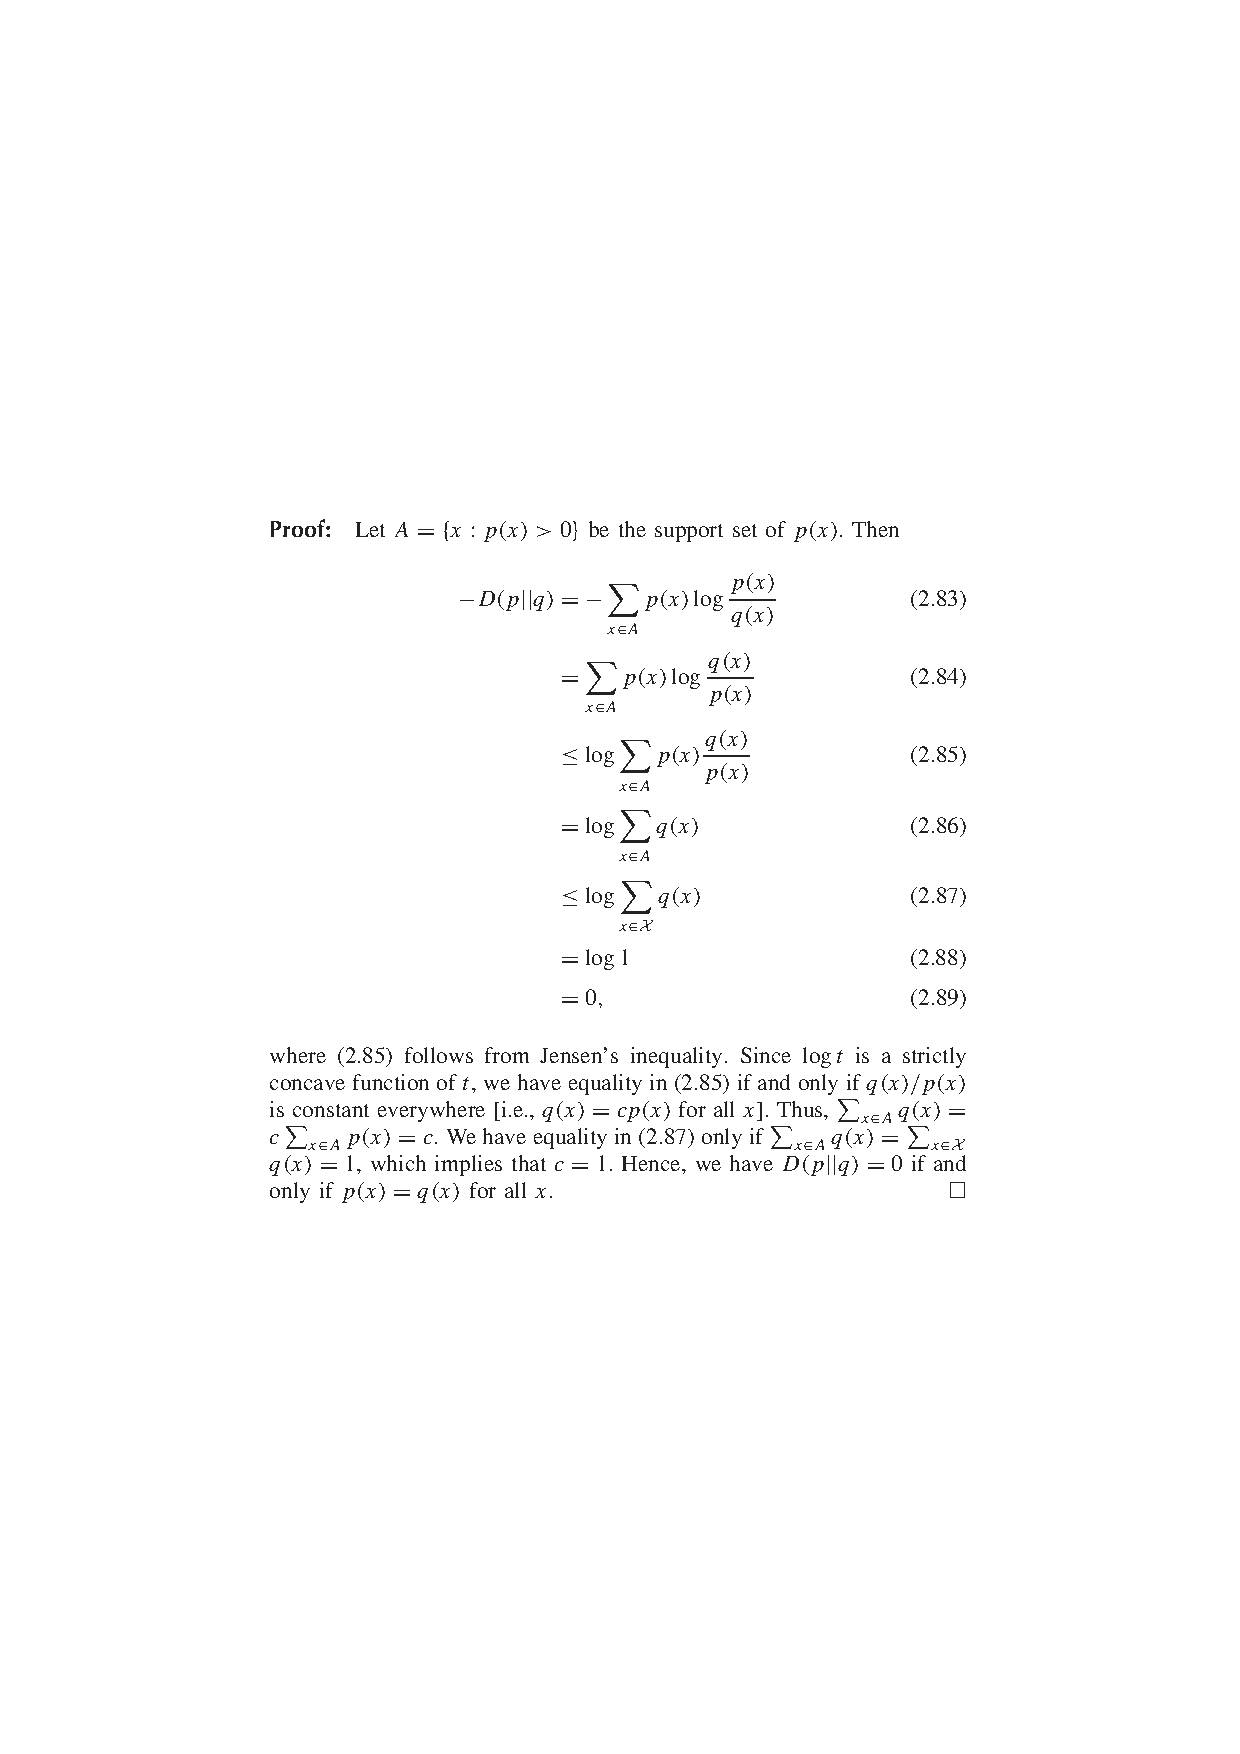
\includegraphics[width=\textwidth]{../imgs/non-negative_DKL.pdf}

\end{theorem}


\end{appendices}


\end{document}